\documentclass[journal]{IEEEtran}

\usepackage[a4paper, left=2cm, right=2cm, top=2cm, bottom=3cm]{geometry}
\usepackage[ngerman]{babel}
\usepackage[utf8]{inputenc}
\usepackage[T1]{fontenc}
\usepackage{hyperref}
\usepackage{graphicx}
\usepackage{lipsum}
\usepackage{xcolor}

\graphicspath{ {./images/} }

\hypersetup{colorlinks=true, allcolors=black}

\title{Proof-of-Concept-Implementierung einer Anwendung mit FIDO2 Support}
\author{
	\IEEEauthorblockN{Mara Schulke \textit{(Matrikel-Nr. 20215853)}}\\
	\IEEEauthorblockA{
		Technische Hochschule Brandenburg \\
		B.Sc. IT Sicherheit \\
		Hardware Sicherheit
	}
}

\begin{document}

\markboth{Hausarbeit Hardware Sicherheit – Mara Schulke}{}
\IEEEspecialpapernotice{
	betreut durch Prof.\ Dr.\ Oliver Stecklina\\
	Sommersemester 2022\\
	Abgabetermin \today
}

\maketitle

\begin{abstract}
	Durch die Implementierung von FIDO2 können bestehende Systeme hinsichtlich
	ihrer Nutzbarkeit und Sicherheit stark verbessert werden und neue Systeme
	grundlegend neue Authentifizierungskonzepte implementieren. Die steigende
	Relevanz zeigt sich durch die Unterstützung großer
	Firmen.~\cite{fidomembers} Durch die Verwendung von ausgereiften
	Abstraktionen über die Protokolle \textit{CTAP} und \textit{WebAuthn} sind
	schnelle und zuverlässige Implementierungen des Standards leicht
	realisierbar.
\end{abstract}

\section{Einleitung}
\IEEEPARstart{A}{\MakeLowercase{uthentifizierung}} ist eines der größten
Probleme, die durch verteilte Systeme entstehen. Es gibt zahlreiche
Möglichkeiten, die Identität einer Gegenseite sicherzustellen allerdings weisen
viele von ihnen Schwachstellen hinsichtlich Man-In-The-Middle-Attacken und
basieren auf der Annahme, dass das System des Nutzers nicht kompromittiert 
wurde. Als eine mögliche Lösung für viele dieser Probleme hat sich FIDO
innerhalb der letzten Jahre zu einem beliebten Standard entwickelt, der von
vielen großen Anbietern wie Facebook, Amazon, Apple, Google, Mozilla,
Microsoft etc.\ bereits unterstützt beziehungsweise implementiert
wird.~\cite{fidomembers}

\section{Der FIDO2 Standard}

FIDO2 steht für \textit{F}ast \textit{ID}entity \textit{O}nline 2 und ist ein
von der FIDO Alliance entwickleter, offener und lizenzfreier Standard für
Hardware-Token gestützte Authentifizierung.

Ein Hardware-Token (kann auch in Form eines Trusted-Plattform-Moduls (TPM) oder
als Teil des Betriebssystems implementiert sein) ist ein physischer Speicher
für die FIDO Schlüsselpaare eines Nutzers. Kernmerkmale, die FIDO2 von
herkömmlicher asymmetrischer Kryptografie unterscheiden, sind beispielsweise
die Isolation der privaten Schlüssel auf dem Hardware-Token, die Notwendigkeit
einer Nutzerinteraktion zum Verwenden eines privaten Schlüssels und die
Generierung von einem Schlüsselpaar pro Online-Dienst.~\cite{ctapspec}

Durch all diese Eigenschaften werden Schlüsselverluste unwahrscheinlicher und
weniger sicherheitskritisch, da selbst bei einem hypothetischen
Schlüsselverlustes der Schaden immer auf einen Online-Dienst begrenzt ist. Die
größte Schwachstelle ist allerdings der physische Diebstahl des
Hardware-Tokens, da dessen Besitz ausreicht für Impersonation-Attacken. Als
Absicherung dagegen kann eine biometrische Authentifizierung erfolgen, bevor
ein privater Schlüssel verwendet werden kann - wie beispielsweise bei FaceID.\

\subsection{Welche Probleme löst FIDO2?}

Die Notwendigkeit für einen solchen Standard hat sich in den letzten Jahren
immer stärker gezeigt, da die klassische Passwort-Authentifizierung durch
zunehmende Rechenleistung und effizientere Angriffe immer unsicherer und
unhandlicher für Nutzer wird. Die minimalen Passwortlängen steigen
dementsprechend an und führen zur Wiederverwendung von gleichen Login-Daten für
mehrere Online-Dienste. Bekannte Lösungen sind die Verwendung von sogenannten
Passwort-Managern um lange und zufällige Passwörter für verschiedenste
Online-Dienste zu verwenden, ohne, dass sich Nutzer diese merken müssen. Solche
Passwort-Manager sind zwar eine Lösung für die sichere Aufbewahrung von langen
Passwörtern, können aber nicht die grundsätzlich durch
Passwort-Authentifizierung eröffneten Angriffsvektoren wie zum Beispiel
Man-In-The-Middle-Attacken. So bald ein Angreifer in den Besitz des geheimen
Wissens (in diesem Fall das Passwort) gelangt, kann dieser uneingeschränkt und
unbegrenzt oft auf das Zielsystem zugreifen, bis der Nutzer seine Daten
ändert (vorausgesetzt, der Angreifer hat dies noch nicht getan).

Durch den Wechsel von Passwort-Authentifizierung auf Zero-Knowledge-Proof
basierte Authentifizierungsmethoden (in diesem Fall
Public-Key-Authentifizierung) lassen sich ganze Angriffsvektoren ausschließen,
da ein kompromittierter Server oder eine kompromitierte Verbindung niemals das
geheime Wissen des Nutzers einem Angreifer zugänglich machen. Das heißt, dass
sich ein Angreifer im Falle einer kompromittierten Verbindung maximal in die
Sitzung des Nutzers einschleichen könnte, allerdings bei der nächsten
Authentifizierung nicht erneut die Identität des Nutzers beweisen könnte und
somit den Zugriff verlieren würde.

Im Falle von FIDO2 kennt nicht einmal der Nutzer selber seine Schlüssel, da
diese auf einem externen Hardware-Token oder TPM gespeichert werden und der
Beweis der Identität durch die Signatur einer vom Authentifizierungs-Server
ausgestellten Challenge erfolgt, die das TPM oder der Hardware-Token intern
durchführen und dem Nutzer nur die Signatur zurückgeben. So stellt selbst ein
kompromittiertes Nutzersystem nur eine temporäre Schwachstelle dar.

\section{Relevante Protokolle: CTAP \& WebAuthn}

Der FIDO2 Standard umfasst hauptsächlich die beiden Protokolle \textit{CTAP}
und \textit{WebAuthn}. Diese unterteilen den gesamten 
Authentifizierungsvorgang in zwei Bereiche:

\textit{Client zu Authenticator} also die Kommunikation zwischen dem
Nutzersystem und dem Hardware-Token und \textit{Client zu Server}, die
Kommunikation zwischen dem Nutzersystem und dem Online-Dienst, bei dem sich der
Nutzer authentifizieren möchte.~\cite{ctapspec, webauthnspec}

\begin{figure}[ht]
	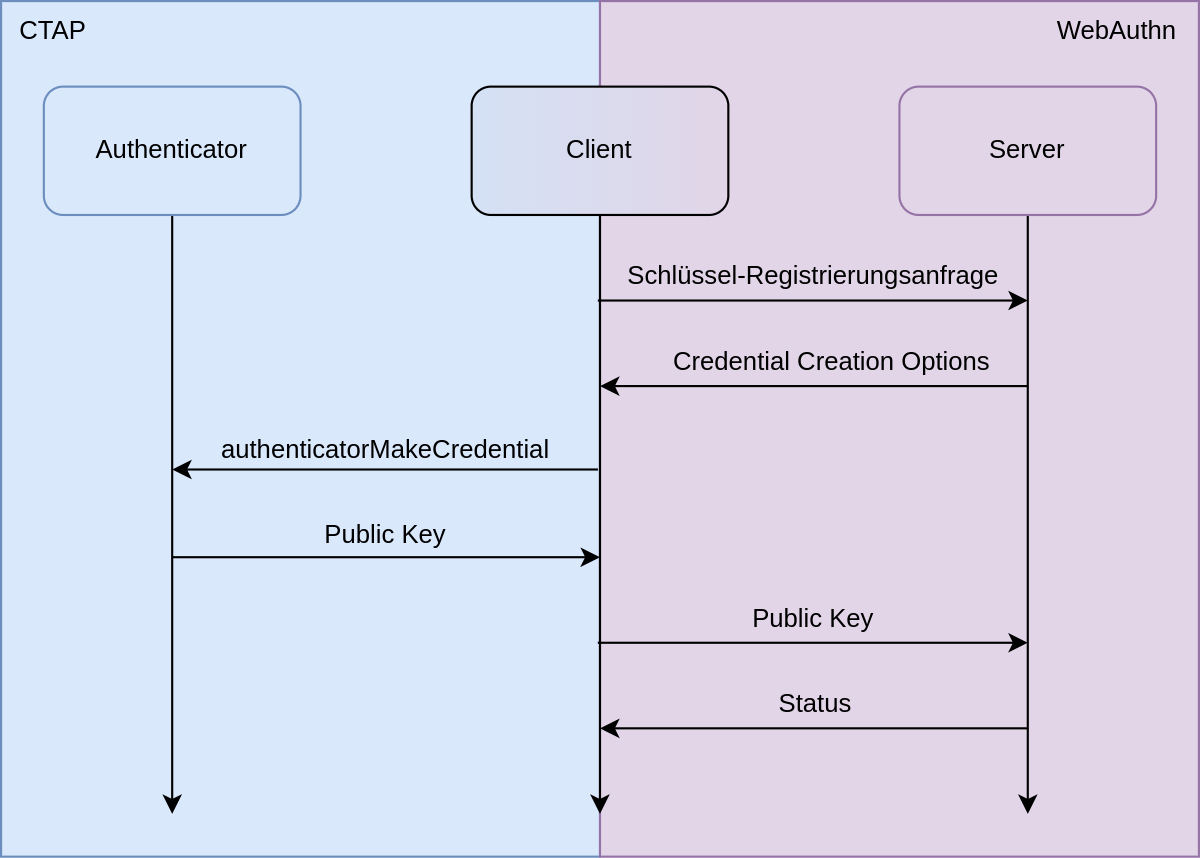
\includegraphics[width=0.5\textwidth]{ctap-webauthn-registration.png}
	\centering
	\caption{Unterteilung des Kommunikationsablaufs in CTAP und WebAuthn am
	beispiel einer Schlüssel-Registrierung}\label{fig:ctap-webauthn}
\end{figure}

\subsection{Gemeinsame Begriffsdefinitionen}

\subsubsection{Relying Party}

Ein Online-Dienst, der den FIDO2 Standard zur Nutzerauthentifizierung
verwendet.

\subsubsection{Authenticator}

Ein externer Hardware-Token oder ein Teil des Betriebssystems (zum Beispiel
über ein TPM implementiert) der FIDO2 Schlüsselpaare verwaltet.

\subsubsection{Credential}

Ein FIDO2 Schlüssel.

\subsubsection{CBOR}

Concise Binary Object Representation, ein Binär-Format zur Darstellung von JSON
Objekten.

\subsection{CTAP}

Das Client-To-Authenticator-Protocol kurz CTAP ist Teil des FIDO2 Standards und
beschreibt den Ablauf der Kommunikation zwischen einem Nutzersystem und dem
Hardware-Token beziehungsweise dem Authenticator.

Neben einer Spezifikation für den Transportlayer / die Nachrichtenstruktur
besteht das Protokoll primär aus der sogenannten ``Authenticator API'' - diese
beschreibt Operationen, die ein Nutzersystem auf einem Authenticator ausführen
kann.~\cite{ctapspec}

Spezifiziert sind die folgenden 6 Operationen:

\begin{enumerate}
	\item \textit{authenticatorMakeCredential} - Schlüsselpaar für eine
		``Relying Party'' erstellen
	\item \textit{authenticatorGetAssertion} - Signatur einer Challenge
	\item \textit{authenticatorGetNextAssertion} - Nächste Signatur der
		Challenge erhalten bei mehreren Schlüsselpaaren
	\item \textit{authenticatorGetInfo} - Informationen über die Fähigkeiten
		des Authenticators abfragen
	\item \textit{authenticatorClientPIN} - Setzt den Authenticator-PIN
	\item \textit{authenticatorReset} - Zurücksetzen auf Werkseinstellungen
\end{enumerate}

Siehe~\cite{ctapspec} Abschnitt 5.

Die im Standard beschriebenen Transportlayer umfassen USB, NFC oder Bluetooth
Low Energy. Für jeden dieser Transportlayer gibt es eigene Mechanismen zum
sicheren Verbindungsaufbau und zur Nachrichtenstruktur.~\cite{ctapspec}

Die JSON Objekte werden innerhalb von \textit{CTAP} mittels dem Datenformat
\textit{CBOR} dargestellt um eine effizientere Codierung zu erhalten und
dennoch die Kompatibilität mit dem weitverbreiteten Standard für
Datenserialisierung zu garantieren.~\cite{ctap, cborspec}

\subsection{WebAuthn}

Ein Server, der das WebAuthn Protokoll implementiert, enthält im wesentlichen
zwei grundlegende Operationen, die jeweils aus mehreren Schritten bestehen.
Diese sind die Registrierung von Sicherheitsschlüsseln (Credentials) und deren
Zuordnung zu einem Nutzeraccount im System der Relying Party und die
Ausstellung beziehungsweise Validierung von WebAuthn Challenges die bei
erfolgreicher Validierung einem Nutzer zugriff auf das System der Relying Party
gibt.

Ein wichtiger Punkt im Zusammenspiel der Spezifikationen und folglich der
Implementierungen der beiden Protokolle \textit{CTAP} und \textit{WebAuthn} ist
die Kompatiblität der Datentypen. So lässt sich die spezifizierte Ausgabe
einer WebAuthn Registrierungs Challenge ohne Veränderung mit der
``authenticatorMakeCredential'' Operation an den Authenticator
weitergeben.~\cite{ctapspec, webauthnspec}

Dies hat zur Folge, dass die Client-Implementierung selbst keine
protokollrelevanten kryptografischen Berechnungen durchführen muss und effektiv
der Server der Relying Party mit dem Authenticator des Nutzers kommuniziert.
Die Client-Implementierung leitet lediglich jeweils die Ausgaben
weiter.~\cite{webauthnspec}

\subsubsection{Registrierung}

Um die Registrierung eines neuen Schlüssels durchzuführen, muss die Relying
Party auf dem Server \texttt{CredentialCreationOptions} für den Nutzer
generieren und an den Client zurücksenden. Diese enthalten Informationen wie
zum Beispiel erlaubte kryptografische Algorithmen, Informationen über den
Nutzer und die Relying Party, ausgeschlossene Authenticator
etc.~\cite{webauthnspec}

Diese Parameter nimmt der Client entgegen und gibt diese dann anschließend an
die \textit{CTAP}-Operation ``authenticatorMakeCredential'' weiter. Der
Authenticator überprüft anschließend, ob er ein Schlüsselpaar erstellen kann,
dass den Anforderungen des Servers entspricht und gibt entweder einen Fehler
oder den öffentlichen Schlüssel an den Client zurück. Dieser wird nun vom
Client an den Server weitergeben und die Registrierung wurde erfolgreich
abgeschlossen.~\cite{ctapspec, webauthnspec}

\subsubsection{Authentifizierung}

Für die Authentifizierung eines Nutzers mittels WebAuthn muss zuerst die
Relying Party eine Challenge für den Client generieren. Diese muss zufällig und
nur einmal gültig sein, um Replay-Attacken zu verhindern. Nachdem der Client
seine Challenge erhalten hat, kann er diese über die CTAP-Operation
``authenticatorGetAssertion'' signieren lassen~\cite{ctapspec} und die
signierte Challenge wieder an den Server zurückgeben. Anschließend überprüft
dieser, ob einer der für den Nutzer hinterlegten Schlüssel verwendet wurde, um
die Challenge zu signieren.~\cite{webauthnspec} War dies der Fall, gilt die
Identität des Nutzers als verifiziert und der Server kann dem Nutzer Zugriff
auf geschützte Ressourcen geben.

\vspace{0.25em}
\rule{0.45\textwidth}{0.4pt}
\vspace{0.5em}

Je nach Kommunikationsprotokoll zwischen dem Client und dem Server muss sich
der Server den Status der Registrierung bzw. Authentifizierung über einzelne
Nachrichten hinweg merken. So sind (auf Nachrichtenebene) verbindungslose
Protokolle wie bspw. HTTPS davon betroffen. Ein bidirektionaler Transport
würde dieses Problem umgehen, da sich der Server nur den Status für die Dauer
der Verbindung merken müsste.

\section{Implementierung des Authetifizierungs-Servers}

\subsection{Zielsetzung}

Ziel der Proof-of-Concept Implementierung ist es eine funktionale,
flüchtige Nutzer-Verwaltung, die optional FIDO2 Schlüssel als zweiten
Login-Faktor unterstützt. Diese soll eine API anbieten, auf der eine
Client-Implementierung aufsetzen kann.

\subsection{Authentifizierungsmechanismus}

Nutzer ohne FIDO2 Schlüssel können sich bei dem Server mittels der Kombination
aus E-Mail und ihrem Passwort authentifizieren und erhalten sofort einen Token
zurück.

Die Nutzer, die einen FIDO2 Schlüssel registriert haben, erhalten nach
initialer Angabe ihrer E-Mail und ihres Passworts eine Aufforderung, ihren
FIDO2 Schlüssel zu verwenden, um letztendlich auch einen Token zu erhalten.

Der Token ist ein JSON-Web-Token der eine Nutzer-Id enthält und ein
Ablaufdatum. Alle Tokens werden mit dem symmetrischen Algorithmus HMAC
(Hash-based Message Authentication Code) signiert.

Alle geschützten beziehungsweise nutzerbezogenen Ressourcen, die dieser Server
vorhält, dürfen nur durch die Mitgabe eines Tokens abgerufen werden. Dieser
muss mit dem \texttt{Authorization}-Header gesetzt werden.

\subsection{Speicherung der Nutzer-Passwörter}

Da bekanntermaßen in Klartext gespeicherte Passwörter eine verheerende
Sicherheitslücke darstellen, speichert der Server nur den Bcrypt-Hash der
Passwörter, die durch einen sogenannten Salt randomisiert werden.

Sowohl der Schlüssel zur Signierung von Tokens als auch der Salt für Bcrypt
müssen in einem realen Anwendungsszenario geheim gehalten werden.

\subsection{Datenstrukturen zur flüchtigen Verwaltung von Nutzern}

Ein Nutzer erhält bei der Registrierung eine eindeutige Id, einen
Verifizierungscode (der in einem realen Anwendungsszenario ggf.\ per E-Mail
versendet werden könnte) und eine leere Liste an FIDO2 Schlüsseln.

Die Nutzer werden in einer HashMap im RAM vorgehalten, eine Datenbankanbindung
des Servers zur Nutzerverwaltung wären bei einem Produktivsystem unabdingbar.

Um die Konsistzenz der Nutzerverwaltung innerhalb des RAM sicherzustellen,
befindet sich die Nutzer-HashMap in einem Mutex, um gleichzeitige ggf.
inkonsistente Schreibvorgänge zu unterbinden.

Bei jeder eingehenden Anfrage wird die Datenstrukturen zur Nutzerverwaltung der
Anfrage zugewiesen, diese hat nun die Garantie, dass sie die einzige Anfrage
ist, die in diesem Moment schreiben kann. Sollten mehrere Anfragen gleichzeitig
eingehen, können diese nur sequenziell abgearbeitet werden. Dies ist zwar
absolut inperformant bei großen Anfragemengen, aber bei einem
Proof-of-Concept-Server mit sehr wenigen Nutzern vertretbar.

\subsection{Implementierung von WebAuthn}

Da die Erstellung von den durch WebAuthn definierten Datenstrukturen und die
kryptografischen Algorithmen nicht trivial zu implementieren sind, gibt es für
gängige Sprachen, die eine Anwendung im Web-Kontext finden, Bibliotheken die
das WebAuthn-Protokoll abstrahiert bereitstellen.

Für Rust ist eine umfangreichere dieser Bibliotheken ``webauthn-rs'',
verfügbar auf GitHub unter der Mozilla-Public-License-2.0:

\url{https://github.com/kanidm/webauthn-rs}

Die Bibliothek lässt sich durch Informationen über den Server konfigurieren:
Es wird eine Relying Party Id und eine registrierbare Domain erwartet, um die
Identität des Servers für die Schlüsselerstellung wiederverwenden zu können.

Nach erfolgreicher Initialisierung gibt es im wesentlichen 4 relevante
Funktionen, mit denen sich der WebAuthn-Flow komplett implementieren lässt:

\subsubsection{start\_securitykey\_registration}
Gibt die Credential-Creation-Options und einen Schlüssel-Registrierungsstatus
für den momentanen Nutzer zurück. Dieser muss persistiert werden.

\subsubsection{finish\_securitykey\_registration}
Nimmt einen Schlüssel-Registrierungsstatus und den generierten Schlüssel und
validiert die Gültigkeit des generierten Schlüssels.

\subsubsection{start\_securitykey\_authentication}
Gibt eine Challenge und einen Schlüssel-Authetifizierungsstatus für den
momentanen Nutzer zurück. Dieser muss persistiert werden.

\subsubsection{finish\_securitykey\_authentication}
Nimmt eine Schlüssel-Authetifizierungsstatus und eine signierte Challenge und
validiert diese gegeneinander.

Somit sind serverseitig alle Voraussetzungen geschaffen, um eine API
bereitzustellen, die WebAuthn unterstützt. Detaillierte Informationen zu den
bereitgestellten Endpunkten finden sich unter Abschnitt~\ref{docs}.

\section{Implementierung der Nutzer-Oberfläche}

\subsection{Zielsetzung}

Ziel ist es, eine beispielhafte Nutzer-Oberfläche zu schaffen, das die unter
Abschnitt~\ref{docs} beschriebene API verwendet, um einen Nutzer-Login mit
FIDO2 zu ermöglichen.

\subsection{Konzept der Oberfläche}

Die Oberfläche ist eine sehr kleine JavaScript Anwendung für die API.\ Folglich
orientieren sich die Aktionen, die der Nutzer in diesem ausführen kann, direkt
an dieser. In der Abbildung~\ref{fig:ui-flow} sind der Ablauf aller möglichen
Nutzeraktionen und die dazugehörigen API-Endpunkte abgebildet.

\begin{figure}[ht]
	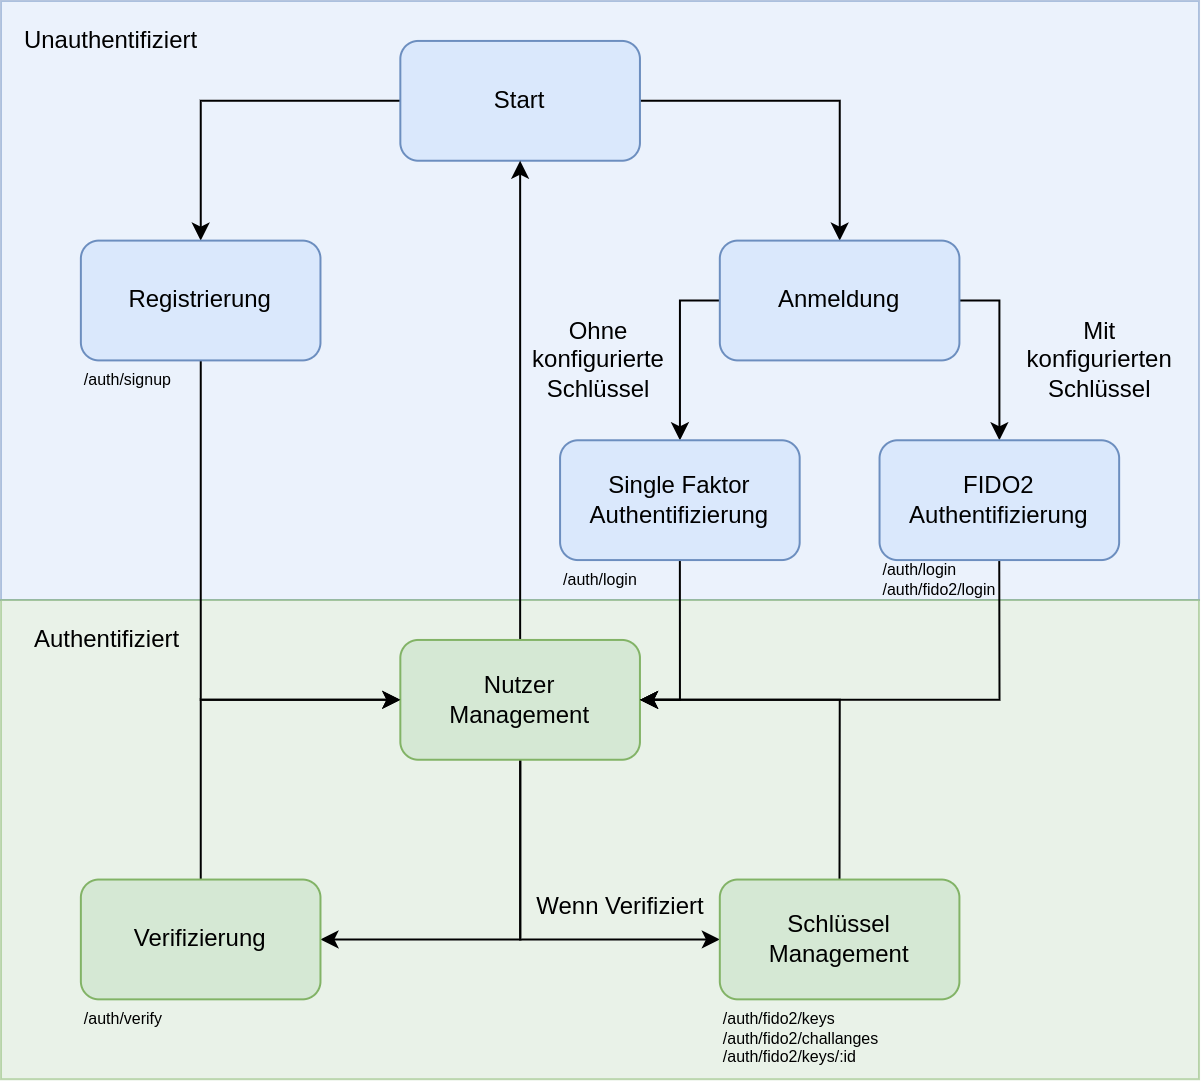
\includegraphics[width=0.5\textwidth]{ui-flow.png}
	\centering
	\caption{Abfolge möglicher Nutzer-Aktionen}\label{fig:ui-flow}
\end{figure}

\subsection{Anwendungs Architektur}

Da der Umfang der Nutzer-Aktionen sich stark in Grenzen hält, gibt es keinen
Grund, eines der komplexeren Frameworks einzusetzen, die typischerweise für
Web-Oberflächen eingesetzt werden. Die einzige externe Bibliothek ist eine
modernere und stabilere Base64 Implementierung als die Browser-native
Alternative.

Das Grundkonzept zum Rendering der Oberfläche ist, einen Anwendungszustand
durch eine pure (also Seiten-Effekt freie) Funktion in HTML zu übersetzen.
Nutzeraktionen können diesen Zustand durch Interaktion verändern und lösen
somit einen neuen Rendervorgang aus. Diese bzw. ähnliche Architekturen findet
sich in Frameworks wie React oder Elm wieder.~\cite{elm}

Der Zustand speichert den Token, Verifizierungsstatus, Ladezustand der
Anwendung und die Liste aller registrierten Schlüssel.

\subsection{Interaktionen}

Die definierten möglichen Interaktionen, die der Nutzer tätigen kann, sind:

\begin{enumerate}
	\item signup
	\item verify
	\item login
	\item logout
	\item addKey
	\item removeKey
\end{enumerate}

Diese werden durch die entsprechenden Bedienfelder der Oberfläche ausgelöst.

\subsection{Implementierung von CTAP}

Da die Nutzer-Oberfläche in JavaScript geschrieben ist und dazu gedacht ist, in
einem Browser-Kontext ausgeführt zu werden, kann die Browser-Implementierung
für CTAP verwendet werden, was die Komplexität der Anwendung drastisch
verringert, da diese Implementierung sehr stark abstrahiert ist.

Im Wesentlichen werden nur zwei der bereitgestellten Funktionen in der gesamten
Nutzer-Oberfläche verwendet:

\begin{enumerate}
	\item navigator.credential.create (führt die Operation
		``authenticatorMakeCredential'' aus)
	\item navigator.credential.get (führt die Operation
		``authenticatorGetAssertion'' aus)
\end{enumerate}

Da die Parameter dieser Funktionen von dem Server bereitgestellt werden, ist
die Implementierung der Kommunikation mit dem Authenticator also sehr trivial.

\section{Technische Dokumentation}\label{docs}

Der Server öffnet den TCP Port 8080 und erwartet eine externe TLS
Terminierung. Tokens können dem Server über den \texttt{Authorization} Header
mitgegeben werden und der \texttt{Content-Type} aller Anfragen und Antworten
ist ausschließlich \texttt{application/json}.

\subsection{/auth/signup - Nutzer erstellen}

\begin{itemize}
	\setlength{\leftskip}{1.5cm}
	\setlength{\itemsep}{0pt}
	\item[Methode:] POST
	\item[Token:] -
	\item[Eingabe:] Credentials \{ email, password \}
	\item[Ausgabe:] UserDetails \{ token, verified, keys \}
	\item[Beschreibung:] Erstellt einen unverifizierten Nutzer ohne FIDO2 Keys.
		Gibt einen Verifizierungscode in den Server-Logs aus (könnte in einem
		echten Szenario per E-Mail verschickt werden).
\end{itemize}

\subsection{/auth/verify - Nutzer verifizieren}

\begin{itemize}
	\setlength{\leftskip}{1.5cm}
	\setlength{\itemsep}{0pt}
	\item[Methode:] POST
	\item[Token:] Notwendig
	\item[Eingabe:] Verification \{ code \}
	\item[Ausgabe:] -
	\item[Beschreibung:] Verifiziert einen Nutzer, falls der Code mit dem bei
		der Registrierung generierten Code übereinstimmt.
\end{itemize}


\subsection{/auth/login - Nutzer anmelden}

\begin{itemize}
	\setlength{\leftskip}{1.5cm}
	\setlength{\itemsep}{0pt}
	\item[Methode:] POST
	\item[Token:] -
	\item[Eingabe:] Credentials \{ email, password \}
	\item[Ausgabe:] UserDetails \{ token, verified, keys \} |
		CredentialRequestOptions 
	\item[Beschreibung:] Gibt dem Nutzer entweder seine UserDetails zurück oder
		stellt eine WebAuthn Authetifizierungs-Challenge die der Nutzer
		signiert bei dem Endpunkt \textit{/auth/fido2/login} enreichen muss,
		falls ein FIDO2 Schlüssel hinterlegt wurde.
\end{itemize}

\subsection{/auth/fido2/login - Nutzer mit WebAuthn anmelden}

\begin{itemize}
	\setlength{\leftskip}{1.5cm}
	\setlength{\itemsep}{0pt}
	\item[Methode:] POST
	\item[Token:] -
	\item[Eingabe:] PublicKeyCredential
	\item[Ausgabe:] UserDetails \{ token, verified, keys \}
	\item[Beschreibung:] Validiert die WebAuthn Challenge des Nutzers mit den
		hinterlegten FIDO2 Schlüsseln und gibt bei erfolgreicher Validierung
		dem Nutzer seine UserDetails zurück.
\end{itemize}

\subsection{/auth/fido2/challenges - WebAuthn Registrierungs Challenge}

\begin{itemize}
	\setlength{\leftskip}{1.5cm}
	\setlength{\itemsep}{0pt}
	\item[Methode:] POST
	\item[Token:] Notwendig
	\item[Eingabe:] -
	\item[Ausgabe:] CredentialCreationOptions 
	\item[Beschreibung:] Startet einen Registrierungsprozess für einen FIDO2
		Schlüssel. Setzt serverseitig den ``Key-Registration-State'' eines
		Nutzers und gibt die Registrierungs-Optionen inklusive einer
		Registrierungs-Challenge zurück.
\end{itemize}

\subsection{/auth/fido2/keys - WebAuthn Registrierung abschließen}

\begin{itemize}
	\setlength{\leftskip}{1.5cm}
	\setlength{\itemsep}{0pt}
	\item[Methode:] POST
	\item[Token:] Notwendig
	\item[Eingabe:] RegisterPublicKeyCredential 
	\item[Ausgabe:] Key \{ id \}
	\item[Beschreibung:] Nimmt die CTAP Ausgabe der
		``authenticatorMakeCredential'' Operation an und ordnet diesen
		Schlüssel dem Nutzer zu.
\end{itemize}

\subsection{/auth/fido2/keys/:id - WebAuthn Schlüssel entfernen}

\begin{itemize}
	\setlength{\leftskip}{1.5cm}
	\setlength{\itemsep}{0pt}
	\item[Methode:] DELETE
	\item[Token:] Notwendig
	\item[Eingabe:] \textit{/:id}
	\item[Ausgabe:] -
	\item[Beschreibung:] Entfernt einen FIDO2 Schlüssel anhand seiner ID.\@
\end{itemize}

\section{Auswertung}

\subsection{Nutzbarkeit}

Das System ist unter Einschränkungen voll funktional und bietet eine
verhältnismäßig gute Nutzbarkeit. Durch die Verwendung eines flüchtigen
Speichermediums (RAM) für die Nutzerverwaltung sind nach jedem Neustart alle
Anwendungsdaten zurückgesetzt. Dies ist für Test-Zwecke absolut in Ordnung und
ließe sich für eine reale Anwendung leicht durch die Implementierung einer
Datenbankanbindung beheben.

Die Nutzer-Oberfläche ist sehr schlicht, lässt aber den Nutzer übersichtlich
alle definierten Interaktionen ausführen. Auch hier ließe sich die
Ausgestaltung der Oberfläche für eine reale Anwendung mit der entsprechenden
Fachexpertise verbessern.

Die Nutzerauthentifizierung an sich verläuft zuverlässig, schnell und
reibungslos. Neben der allgemeinen Dateneingabe (E-Mail und Passwort) besteht
die Signierung der Challenge lediglich aus einem Tippen auf den Authenticator.
Dies allein bietet ein deutlich verbessertes Erlebnis im Vergleich zu
SMS-Tokens oder One-Time-Passwords als zweiten Faktor (vorausgesetzt der
Authenticator befindet sich in der Nähe des Systems oder ist sogar bereits
angeschlossen).

\subsection{Risiken}

Die Hauptrisiken des momentanen Systems ist die fehlende Passwortvalidierung
und der fehlende Zwang, einen FIDO Schlüssel bei der Registrierung zu
hinterlegen. So ist es momentan möglich, einen Nutzer mit einem schwachen
Passwort anzulegen und keinen Schlüssel zu registrieren. Dies ließe sich
gegebenenfalls auch durch Anpassung des Authentifizierungs bzw.
Registrierungsprozesses beheben.

Unter der Annahme, dass eine Schlüssel-Registrierung verpflichtend sei, wäre
ein Angriff auf einen Nutzeraccount nur noch durch physikalische Entwendung des
Hardware-Tokens möglich und dementsprechend unwahrscheinlich. Somit kann unter
dieser Annahme das System als sicher angesehen werden.

\subsection{Mögliche Verbesserungen}

Als abschließende Verbesserung wäre ein Umstellen auf
Single-Faktor-Authentifizierung mit dem Hardware-Token hinsichtlich des
Nutzer-Erlebnises empfehlenswert (Sicherheitsimplikationen außer Acht
gelassen). 

Eine alternative Möglichkeit könnten weiterhin die Verwendung von zwei Faktoren
sein, allerdings unter der Bedingung, dass das Passwort lediglich zur
einrichtung neuer Systeme abgefragt wird und sonst ein Single-Faktor-Login mit
dem Hardware-Token möglich ist.

Des Weiteren ist es bei Hardware Tokens - deren physikalischer Verlust nicht
gänzlich auszuschließen ist - ratsam, einen Backup Token zu besitzen und diesen
bei jedem Online-Dienst als Backup Token zu hinterlegen, um einen
Schlüsselverlust abfangen zu können. Eine bekannte Alternative zu einem zweiten
Hardware Token wären auch sogenannte Backup Codes, die bei Schlüsselverlust
einmaligen Zugriff gewähren.

All diese ausgereiften Konzepte werden in der momentanen
Proof-of-Concept-Implementierung noch außer Acht gelassen, ließen sich
allerdings leicht mit geringem zusätzlichen Aufwand hinzufügen.

\listoffigures

\bibliographystyle{IEEEtran}
\bibliography{IEEEabrv,references}

\section*{Anhang}

\subsection*{Quellcode der Implementierung}

\url{https://github.com/mara214/fido2-auth}

\subsection*{Zur Entwicklung verwendeter Authenticator}

\url{https://store.google.com/de/product/titan_security_key}


\end{document}
